\documentclass[10pt, a4paper]{article}
\usepackage[a4paper, top=20mm, left=18mm, right=18mm, bottom=20mm]{geometry}
\usepackage{hyperref}
\usepackage[sf]{titlesec}
\usepackage{listings}
\usepackage{graphicx}
\usepackage{float}
\usepackage{color}
\hypersetup{hidelinks = true}
\definecolor{codegrey}{rgb}{0.95, 0.95, 0.96}
\lstset{
	backgroundcolor = \color{codegrey}
}
\begin{document}
{\fontfamily{cmss}\selectfont

\title{\vspace{-20mm}CMPUT 291 - Mini Project 1 Design Document}
\date{}
\maketitle
\vspace{-20mm}
\section{Overview}\label{OV}
The following python application is used to connect to an existing SQLite3 database storing enterprise data. The application is run through the terminal, and is operated with simple command line inputs. For informatino on connecting to a database and running the application, see \emph{\nameref{UG}}.

Users with valid login credentials will be provided access to various functions to interact, view, and update the data stored in the database. Depedning on their user type (determined by the databes) the functionalities include: \emph{Register a birth, Register a marriage, Renew a vehicle registration, Process a bill of sale, Process a payment, Get a driver abstract, Issue a ticket, Find a car owner}. For speceifics on these functions and their operations, see \emph{\nameref{SD}}.

\subsection{User Guide}\label{UG}
To launch the application, run the following command from the directory holding the source code:
\begin{lstlisting}
    $ python3 db.py
\end{lstlisting}
To connect to a database, enter the path to the database when prompted (a):
\begin{lstlisting}
    Enter path of database: path/to/database.db
\end{lstlisting}
Once the database connection is successfuly established, the user will be prompted to enter their username and password (b), for example:
\begin{lstlisting}
    Username: admin123
    Password: pwd12345
\end{lstlisting}
Depending in the user type (agent or officer), numerical options will appear on screen. Enter the number of the task you wish to perform, and follow the on-screen instructions. For further information regardin the options, see \emph{\nameref{SD}}. 

At the main user menu, the user can logout by entering the `0' key, which will return the application to the login screen. The application will remain connected to the database entered at launch, and other useres are able to login from here.

The user can return to the main menu from any point within performing a task by hitting ctrl-d. Note: if a new entity was commited to the database or before hitting crtl-d, \textbf{this action will be saved in the database}, i.e. if a parent needs to be registered in order to register a birth, and this step is completed, and the user exits to the main menu before completeing the birth registration process, the newly registered parent will reain in the database. 

At the login in screen, the application can be exited by pressing crtl-d.

\begin{figure}[H]
\centering
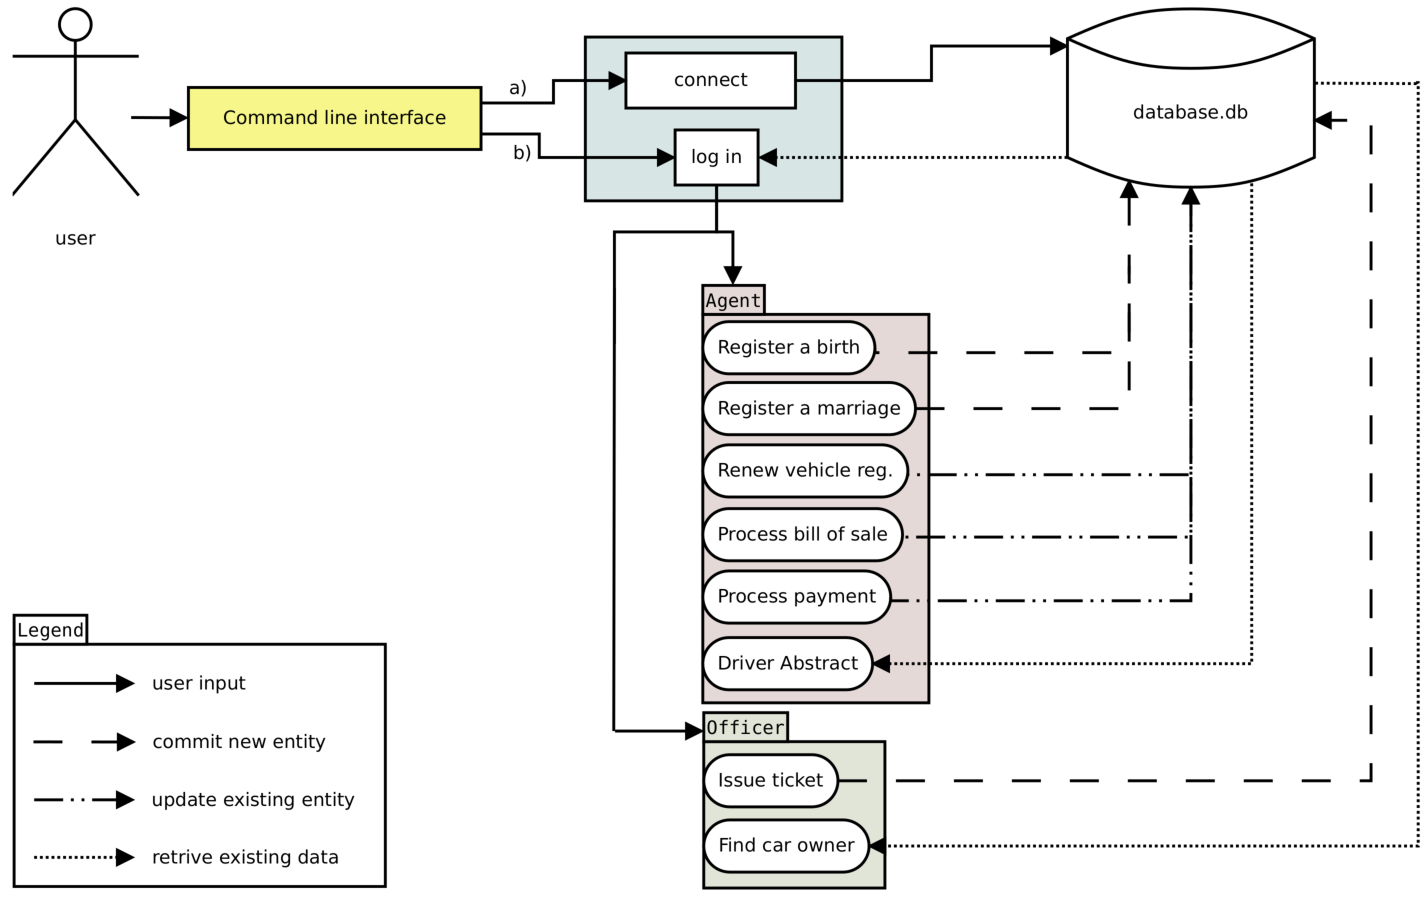
\includegraphics[height=8cm]{Diagram1.pdf}\label{fig}
\caption{Diagram showing flow of data between application user, application functions, and the connceted database.}
\end{figure}

\section{Software Design}\label{SD}
\begin{itemize}

\item User Menu
	\begin{quotation}
	\noindent After a successful log in, the user is provided a menu with numbered options. 
	\end{quotation}

\item Register a birth
	\begin{quotation}
	\noindent Registers a new person into \emph{persons} table and a new birth record in \emph{births} table. Prompts user to enter child's first and last name, birth gender, mother's first and last name, father's first and last name, and the child's birth date and birth place. Registration place is automatically set to the user's city, and registration date is set to today's date. Child inherits mother's address and phone number. In the case where the mother or father do not exist in the database, the user has the option to register them, then continue wuth the birth registration. 
	\end{quotation}
\item Register a marriage
\item Renew a vehicle registration
\item Process a bill of sale
\item Process a payment

\item Get a driver abstract
	\begin{quotation}
	\noindent Promts user to enter first and last name of a registered person to display their driver abstract. If the name entered is not found, the user has the option to renter the name, or return to the main menu. The driver abstract consists of: ticket counts for lifetime and last two years, demerit notices and points for lifetime and last two years. The agent has the option to view a detailed ticket history by entering the t/T key. Initially five tickets are displayed in order from most recent to oldest, with an option to display 5 more until the end of the history.
	\end{quotation}

\item Issue a ticket
\item Find a car owner
\end{itemize}

\section{Testing Strategy}\label{TS}
Functions of the software were tested as they were developed, and then again when the entire development process was completed. For each of the functionalities, the follwoing cases were tested:
\begin{itemize}
\item{\emph{Register a birth}: Both parents in db; only one parent in db; no parents in db; mother with Null values}
\item{\emph{Register a marriage}: partners not in db}
\item{\emph{Renew a vehicle registration}: regno not found}
\item{\emph{Process a bill of sale}: }
\item{\emph{Process a payment}: invalid tno; invalid payment amount (i.e. over paying a ticket)}
\item{\emph{Get a driver abstract}: driver not found in db}
\item{\emph{Issue a ticket}: regno not found; violation date specified; violation date not specified }
\item{\emph{Find a car owner}: }
\end{itemize}

\section{Group Break-down Strategy}\label{GS}
The group work strategy must list the break-down of the work items among partners, both the time spent (an estimate) and the progress made by each partner, and your method of coordination to keep the project on track. The design document should also include a documentation of any decision you have made which is not in the project specification or any coding you have done beyond or different from what is required.

\end{document}
